\subsection{Experiment 1: Selective Updating on Unresolved Questions}
\label{sec:exp1}

Experiment~1 tests whether forecasts respond to the stated direction and relevance
of new evidence. Because most directional packets state their implication, a model
can pass without deriving a causal path. It must still distinguish directional
evidence from topically related controls.

\begin{figure}[t]
\centering
\begin{subfigure}[c]{0.49\textwidth}
\centering
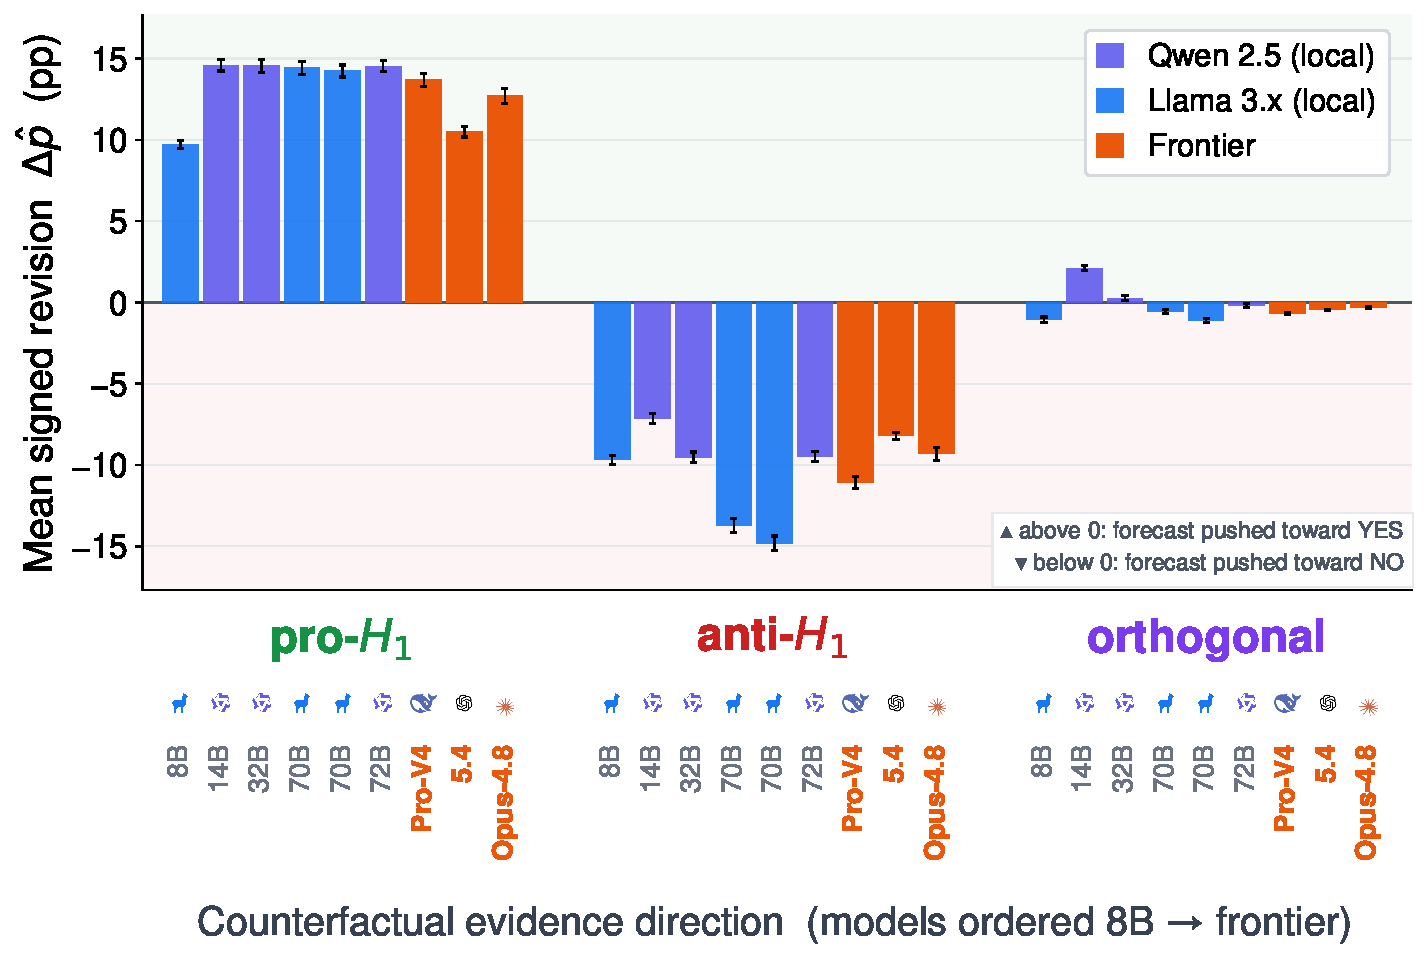
\includegraphics[width=\linewidth]{figures/exp1_direction_selective_updating.pdf}
\caption{}
\label{fig:exp1-bars}
\end{subfigure}\hfill
\begin{subfigure}[c]{0.48\textwidth}
\centering
\footnotesize
\setlength{\tabcolsep}{4pt}
\begin{tabular*}{\linewidth}{@{}l@{\extracolsep{\fill}}ccc@{}}
\toprule
\textbf{Model} & \textbf{Sens.}$\uparrow$ & \textbf{$|\Delta p|_{\rm D/O}$} & \textbf{EHC$_{\geq3}$}$\uparrow$ \\
\midrule
\micon{claude.png}~Opus~4.8 & \cellcolor{heatgreen}$24.0\times$ & \cellcolor{heatgreen}$11.1/0.5$ & \cellcolor{heatgreen}.990 \\
\micon{openai.png}~GPT-5.4 & \cellcolor{heatyellow}$8.2\times$ & \cellcolor{heatyellow}$9.5/1.2$ & \cellcolor{heatgreen}.987 \\
\micon{deepseek.png}~V4-Pro & \cellcolor{heatyellow}$8.9\times$ & \cellcolor{heatyellow}$12.7/1.4$ & \cellcolor{heatyellow}.977 \\
\midrule
\micon{llamma.pdf}~3.3-70B & \cellcolor{heatyellow}$6.4\times$ & \cellcolor{heatyellow}$14.5/2.3$ & \cellcolor{heatyellow}.965 \\
\micon{llamma.pdf}~3.1-70B & \cellcolor{heatorange}$4.6\times$ & \cellcolor{heatorange}$15.1/3.3$ & \cellcolor{heatyellow}.961 \\
\micon{qwen.pdf}~2.5-72B & \cellcolor{heatorange}$4.2\times$ & \cellcolor{heatorange}$12.6/3.0$ & \cellcolor{heatyellow}.963 \\
\micon{qwen.pdf}~2.5-32B & \cellcolor{heatorange}$3.2\times$ & \cellcolor{heatorange}$12.6/4.0$ & \cellcolor{heatyellow}.964 \\
\micon{qwen.pdf}~2.5-14B & \cellcolor{heatorange}$2.9\times$ & \cellcolor{heatorange}$11.8/4.1$ & \cellcolor{heatorange}.943 \\
\micon{llamma.pdf}~3.1-8B & \cellcolor{heatred}$1.9\times$ & \cellcolor{heatred}$11.5/5.9$ & \cellcolor{heatred}.887 \\
\bottomrule
\end{tabular*}
\caption{}
\label{fig:exp1-table}
\label{tab:consistency}
\end{subfigure}
\caption{\textbf{Direction-selective updating across nine models and 30,094 valid update
records.} \textbf{(a)} Mean signed forecast revision by counterfactual direction;
error bars are standard errors. \textbf{(b)} Packet selectivity and directional
correctness. Sensitivity is mean directional divided by mean orthogonal absolute
revision; D/O reports those means in percentage points. EHC is the conditional
directional-correctness rate among movements of at least three percentage points.
Colors progress from red through orange and yellow to green
using the descriptive bands defined in Methods. Output-field compliance and a
0/1/3/5-pp threshold sweep appear in Appendix~\ref{app:exp1-threshold-robustness}.}
\label{fig:exp1-updating}
\end{figure}

\textbf{Models distinguish direction-bearing packets from topical controls.}
Frontier sensitivity ranges from $8.2\times$ to $24.0\times$: the same agents move
farther under pro- and anti-$H_1$ packets than under orthogonal packets. Every
scale-valid local model shows the same ordering, with sensitivity from
$1.9\times$ to $6.4\times$.
The result is therefore not confined to the frontier systems, although selectivity
is weaker in the smaller open-weight models.

\textbf{Directional movements usually follow the stated sign.}
Across 30,094 valid updates, conditional EHC ranges from .887 to .990
(Figure~\ref{fig:exp1-updating}), and all three frontier agents exceed .97.
Their unconditional directional correctness is 97.3--98.4\%; the 3-point
conditional metric omits 6.9--18.1\% of directional updates that move less than the
threshold. Because this measure is near ceiling, it serves as a directional
guardrail rather than the primary model comparison.

These results reject an update policy that reacts equally to any
news-like text about the market. They remain compatible with reading the packet's
explicit polarity and applying a learned numerical shift. Experiment~2 instead
makes the qualitative cue informative only through numerical reference cases.
